\documentclass{beamer}

\usepackage{amsmath, amsfonts, amssymb}
\usepackage{booktabs}
\usepackage{graphicx}
\usepackage{cmbright}
\usepackage{fontspec}

\beamertemplatenavigationsymbolsempty
\usetheme{metropolis}

\DeclareMathOperator*{\argmax}{arg\,max}

\AtBeginSection[]{
  \begin{frame}
  \vfill
  \centering
  \begin{beamercolorbox}[sep=8pt,center,shadow=true,rounded=true]{title}
    \usebeamerfont{title}\insertsectionhead\par%
  \end{beamercolorbox}
  \vfill
  \end{frame}
}

\title{Impulse Response Estimation by Smooth Local Projections (SLPs)}
\subtitle{Matthew Kielar \& Elijah Adrian}
\date[]{ECON 622 001}

\begin{document}

\begin{frame}[plain, noframenumbering]
    \titlepage
\end{frame}

\begin{frame}{Overview}

    Estimation of impulse response functions (IRFs) is a cornerstone of modern macroeconomic analysis \bigskip

    \begin{itemize}
        
        \item Illustrate how different shocks propagate throughout the real economy
        \item Useful for constructing counterfactuals or "what-if" analysis

    \end{itemize} \bigskip

    Impulse response estimation usually tends to be handled by vector autoregression models. Is there
    possibly a better way?

\end{frame}

\begin{frame}{Local Projections (LPs)}

    Jorda (2005) proposed local projections (LPs) as an alternative method for estimating
    impulse responses. \bigskip

    Basic idea: Given variables $y_t$, instead of estimating one model just regress future
    values of $y$ on current values at each horizon $k$. \bigskip
    
    At each horizon, run the following OLS regression:

    \begin{equation*}
        y_{t+k} = \alpha_k + \beta_k x_t + \gamma'_k r_t + \sum_{k=1}^p \delta'_k w_{t-k} + \varepsilon_{t+k}
    \end{equation*}

    where $x_t$ is the shock variable and $w_t$ is a vector of control variables, usually lags of
    the endogenous variables. \bigskip
   
    Under this setup, $\hat{\beta}_k$ captures the impulse response at horizon $k$. 

\end{frame}

\begin{frame}{Why LP?}

    VARs are efficient, but sensitive to misspecification. Incorrect specification at
    the first lag results in errors being iterated forward. \bigskip

    Local projections are considerably more robust in this regard. \bigskip 

    Estimation of separate OLS equations for each horizon $\to$ errors don't propagate
    across horizons. \bigskip 

    \begin{itemize}

        \item Since IRFs are just vectors of scalar values, can apply different smoothing methods
        \item More flexible estimation options
        
    \end{itemize} \bigskip

    Consistency: If the true DGP is VAR(p) and LP estimator includes the same lag structure, then
    $\hat{\delta}_k \to_p A_1^k$ as $T \to \infty$.

\end{frame}

\begin{frame}{B-Splines}

    A B-spline is a collection of piecewise polynomials $B_{i,p}(x)$ in a variable $x$ \bigskip

    \begin{itemize}
        \item Values of $x$ where the ``pieces'' are connected are known as the ``knots'' of the spline
        \item Smoothness determined by the degree $p$ of the polynomials  
        \item Nonzero only on a small interval defined by the knots
    \end{itemize} \bigskip

    The splines are constructed as a weighted sum of these basis functions, with weights determined
    from the data \bigskip

    General representation: $f(x) \approx \sum_{k=1}^K b_k B_k(x)$

\end{frame}

\begin{frame}{B-Splines}

    \begin{figure}[h!]
        \centering
        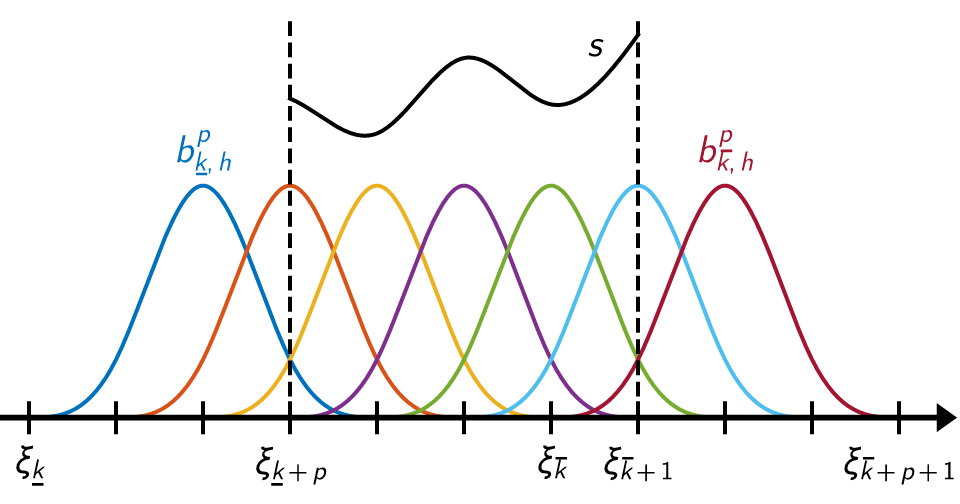
\includegraphics[width=0.85\textwidth]{uniform-b-splines.png}
    \end{figure}

\end{frame}

\begin{frame}{Smooth Local Projections (SLP)}
   
	Barnichon and Brownlees (2019) propose utilising B-splines to smooth the sequence of LP
    estimates $\hat{\beta}_k$ \bigskip

	IRFs estimated by LP can deviate from the true IRF $\to$ smoothing can bring estimated
    impulse responses closer to the actual DGP \bigskip

	B-splines are a pretty well-suited smoothing method here:

	\begin{itemize}
		
		\item Flexible and data-adaptive (easily fine-tuned via knots or polynomial degree)
		\item Computationally efficient due to local control properties 

	\end{itemize}

\end{frame}

\begin{frame}{Smooth Local Projections (SLP)}

    Overview of the SLP procedure:

    \begin{enumerate}
    
        \item Form a B-spline basis $\mathbf{B}$

        \item At each horizon $k$, evaluate the basis $\mathbf{B}$ to get $\mathbf{b}(k)$ and form $\tilde{\mathbf{X}}_k = \mathbf{b}(k)' x_t$

        \item Stack all the relevant variables into a block-diagonal matrix

        \item Estimate the B-spline coefficients in one-shot via L2 regularisation

    \end{enumerate}

\end{frame}

\begin{frame}{Where does our project fit in?}

    Plan: write a generic python implementation of the SLP estimation procedure

    What we've got so far:

    \begin{itemize}
        \item Generic methods to estimate local projections
        \item B-splines and some other smoothers (kernel and LOESS)
    \end{itemize}

    Some stuff we want to add (subject to revision):

    \begin{itemize}
        \item Some basic plotting functionality
        \item Expository vignettes comparing SLP to VAR
        \item Throwing together a Python package for public use (ambitious)    
    \end{itemize}

\end{frame}

\end{document}
